\section{Analytical Solutions}
	\subsection{Rectangular quantum well}
		\begin{figure}[!h]
			\centering
			\begin{tikzpicture}[scale=4,cap=round,>=latex]
	\draw [<->] (-2, 1.5) -- (-2, 0) -- (1.5, 0);
	\node [left] at (-2, 1.5) {$U$};
	\node [below] at (1.5, 0) {$z$};
	
	\draw [line width=1.5] (-2, 1) -- (-1, 1) -- (-1, 0) -- (0, 0) -- (0, 1) -- (1, 1);
	\draw [dashed] (-1, 1) -- (-1, 1.5);
	\draw [dashed] (0, 1) -- (0, 1.5);
	
	\node [left] at (-2, 1) {$U_0$};
	\node [below] at (-1, 0) {$-\frac{d}{2}$};
	\node [below] at (0, 0) {$\frac{d}{2}$};
	
	\node at (-1.5, 1.2) {I};
	\node at (-0.5, 1.2) {II};
	\node at (0.5, 1.2) {III};										
\end{tikzpicture}
			\caption{Finite rectangular quantum well}
		\end{figure}
		
		\begin{equation}
			\hat{H} = \frac{\hbar}{2m} \frac{\partial^2}{\partial z^2} + U(z)
		\end{equation}
		
		\begin{align}
			\text{II:}&\qquad E\Psi = \frac{\hbar}{2m} \frac{\partial^2}{\partial z^2}\Psi \\
			\text{I \& III:}& \qquad E\Psi = \frac{\hbar}{2m} \frac{\partial^2}{\partial z^2}\Psi + U_0\Psi 
		\end{align}
				
		Solutions for each area:
		\begin{align}
			\text{I:}&\qquad \Psi = A e^{+ik'z} + B e^{-ik'z} \\
			\text{II:}&\qquad \Psi = C e^{+ikz} + D e^{-ikz} \\
			\text{III:}&\qquad \Psi = F e^{+ik'z} + G e^{-ik'z} \\
			&\qquad k = \sqrt{\frac{2mE}{\hbar^2}};\qquad k' = \sqrt{\frac{2m(E-U_0)}{\hbar^2}}
		\end{align}
		For $E < U_0$, $k'$ is imaginary, meaning that
		\begin{align}
			\lim_{z \to -\infty} Ae^{+ik'z} = \lim_{z \to -\infty} Ae^{-sz} = \infty \\
			\lim_{z \to \infty} Ge^{-ik'z} = \lim_{z \to \infty} Ae^{sz} = \infty
		\end{align}
		Which is not physical, meaning that 
		\begin{equation}
			A = G = 0
		\end{equation}
		We have bounadary conditions at $z = -\frac{d}{2}$ and $z = \frac{d}{2}$:
		\begin{align}
			\Psi_I = \Psi_{II}|_{z=-\frac{d}{2}};&\qquad  \Psi_I' = \Psi_{II}'|_{z=-\frac{d}{2}} \\
			\Psi_{II} = \Psi_{III}|_{z=\frac{d}{2}};&\qquad  \Psi_{II}' = \Psi_{III}'|_{z=\frac{d}{2}}
		\end{align}
		Which can be written as:
		\begin{align}
			\kappa = ik' =& \sqrt{\frac{2m(U_0-E)}{\hbar^2}} \\
			Be^{-\kappa\frac{d}{2}} = Ce^{-ik\frac{d}{2}} + De^{+ik\frac{d}{2}}&\\
			-B\kappa e^{-\kappa\frac{d}{2}} &= ikCe^{-ik\frac{d}{2}} - ikde^{+ik\frac{d}{2}}\\
			Fe^{-\kappa\frac{d}{2}} = Ce^{+ik\frac{d}{2}} + De^{-ik\frac{d}{2}}&\\
			-F\kappa e^{-\kappa\frac{d}{2}} &= ikCe^{+ik\frac{d}{2}} - ikde^{-ik\frac{d}{2}}\\
		\end{align}
		Or in matrix form:
		\begin{equation}
			\begin{pmatrix}
			e^{-\kappa\frac{d}{2}}			&	-e^{-ik\frac{d}{2}}	&	-e^{ik\frac{d}{2}}	&	0 \\ 
			0	&	-e^{-ik\frac{d}{2}}	&	-e^{-ik\frac{d}{2}}	&	e^{-\kappa \frac{d}{2}} \\
			-\kappa e^{-\kappa \frac{d}{2}}	& -ike^{-ik\frac{d}{2}}	& +ike^{ik\frac{d}{2}}	& 0 \\
			0	& +ike^{ik\frac{d}{2}}	& -ike^{ik\frac{d}{2}}	& 	-\kappa e^{-\kappa\frac{d}{2}}	& \\
			\end{pmatrix}
			\begin{pmatrix}
			B \\
			C \\
			D \\
			F \\
			\end{pmatrix}
			=
			\begin{pmatrix}
			0 \\
			0 \\
			0 \\
			0 \\
			\end{pmatrix}			
		\end{equation}
		\hl{Direct solution?}
		Since our system is symmetric, we can simplify the system of equations:
		
		\begin{align}
			|\Psi|^2_{-\frac{d}{2}} =& |\Psi|^2_{\frac{d}{2}} \Rightarrow\\
			\Psi(z) = \Psi(-z) \qquad\text{or}&\qquad \Psi(z) = -\Psi(-z)
		\end{align}
		Which means that our system can have either symmetric or antisymmetric solutions:
		\begin{align}
			\Psi_{II}& = C e^{ikz} + D e^{-ikz} = C' \cos(kz) + D' \sin(kz) \\
			\Psi_{I}& = B e^{-\kappa z} \\
			\Psi_{III}& = F e^{\kappa z} \\		
		\end{align}
		Where $C'\cos(kz)$ and $A=F$ correspond to symmetric solutions and $D' \sin(kz)$ and $A = -F$~--- to antisymmetric solutions.
		
		\subsubsection{Symmetric solutions}
		
		\begin{align}
			Be^{-\kappa \frac{d}{2}} &= C' \cos(\frac{kd}{2}) \\
			\kappa Be^{-\kappa \frac{d}{2}} &= kC' \sin(\frac{kd}{2})			
		\end{align}
		Or in matrix form:
		\begin{equation}
		\begin{pmatrix}
		e^{-\kappa \frac{d}{2}}			&	-\cos{\frac{kd}{2}}	\\ 
		\kappa e^{-\kappa \frac{d}{2}}	&	-k\sin{\frac{kd}{2}}	\\
		\end{pmatrix}
		\begin{pmatrix}
		B \\
		C' \\
		\end{pmatrix}
		=
		\begin{pmatrix}
		0 \\
		0 \\
		\end{pmatrix}			
		\end{equation}
		This system has non-trivial solutions when the determinant of the matrix is equal to zero:
		\begin{align}
			\begin{vmatrix}
				e^{-\kappa \frac{d}{2}}			&	-\cos{\frac{kd}{2}}	\\ 
				\kappa e^{-\kappa \frac{d}{2}}	&	-k\sin{\frac{kd}{2}}	\\
			\end{vmatrix}
			=& -e^{-\kappa\frac{d}{2}} k\sin{\frac{kd}{2}} + \kappa e^{-\kappa \frac{d}{2}} \cos{\frac{kd}{2}} =\\
			=& -k\sin(\frac{kd}{2}) + \kappa\cos(\frac{kd}{2}) = 0 \\
			\frac{k}{\kappa} =& \cot(\frac{kd}{2}) \label{symtranceq}
		\end{align}
		
		With solutions to \ref{symtranceq} defining the number of bound states in the quantum well. 
		\begin{figure}[!h]
			\centering
			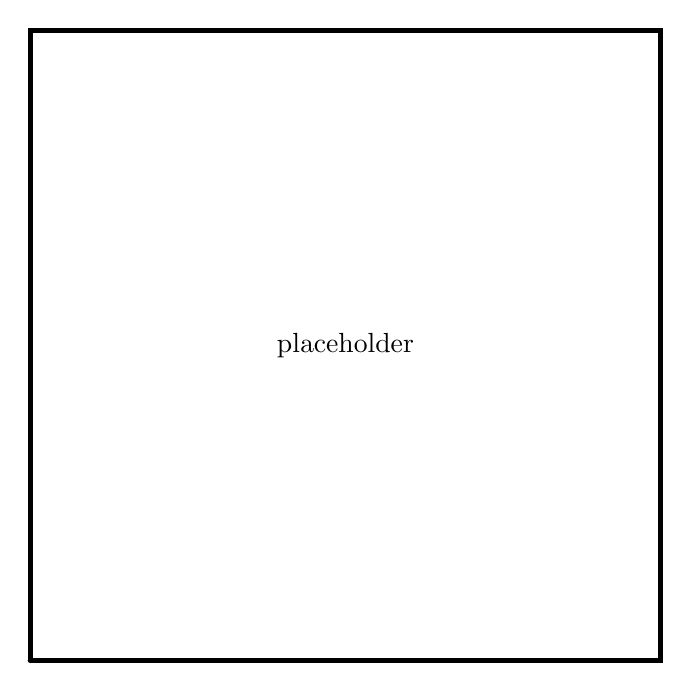
\begin{tikzpicture}[scale=2,cap=round,>=latex]
	\draw [line width=2] (-2, -2) -- (-2, 2) -- (2, 2) -- (2, -2) -- (-2, -2);
	
	\node at (0, 0) {placeholder};
\end{tikzpicture}
			\caption{Graphical solution to \ref{symtranceq}}
		\end{figure}
		
		In the limit case of $U_0 \rightarrow \infty$,
		\begin{align}
			\frac{k}{\kappa} =& \cot(\frac{kd}{2}),\qquad \kappa \rightarrow \infty \Rightarrow \\
			\cot(\frac{kd}{2}) =& 0 \Rightarrow\qquad	\cos(\frac{kd}{2}) = 0 \Rightarrow\\
			\frac{kd}{2} =& \frac{\pi}{2} + \pi n \\
			k_n =& \frac{\Pi + 2\pi n}{d} \\
			E_n =& \frac{\hbar^2}{2m}\frac{1}{d^2}\left(\pi + 2\pi n\right)^2
		\end{align}
		Which corresponds to the symmetric solutions found earlier to the infinite quantum well problem.
		
		\subsubsection{Antisymmetric solutions}
		
		\begin{align}
			Be^{-\kappa \frac{d}{2}} &= D' \sin(\frac{kd}{2}) \\
			\kappa Be^{-\kappa \frac{d}{2}} &= -kD' \cos(\frac{kd}{2})			
		\end{align}
		Or in matrix form:
		\begin{equation}
		\begin{pmatrix}
		e^{-\kappa \frac{d}{2}}			&	-\sin{\frac{kd}{2}}	\\ 
		\kappa e^{-\kappa \frac{d}{2}}	&	k\cos{\frac{kd}{2}}	\\
		\end{pmatrix}
		\begin{pmatrix}
		B \\
		D' \\
		\end{pmatrix}
		=
		\begin{pmatrix}
		0 \\
		0 \\
		\end{pmatrix}			
		\end{equation}
		This system has non-trivial solutions when the determinant of the matrix is equal to zero:
		\begin{align}
			\begin{vmatrix}
				e^{-\kappa \frac{d}{2}}			&	-\sin{\frac{kd}{2}}	\\ 
				\kappa e^{-\kappa \frac{d}{2}}	&	k\cos{\frac{kd}{2}}	\\
			\end{vmatrix}
			=& e^{-\kappa\frac{d}{2}} k\cos{\frac{kd}{2}} + \kappa e^{-\kappa \frac{d}{2}} \sin{\frac{kd}{2}} =\\
			=& k\cos(\frac{kd}{2}) + \kappa\sin(\frac{kd}{2}) = 0 \\
			\frac{k}{\kappa} =& -\tan(\frac{kd}{2}) \label{antisymtranceq}
		\end{align}
		
		With solutions to \ref{antisymtranceq} defining the number of bound states in the quantum well. 
		\begin{figure}[!h]
			\centering
			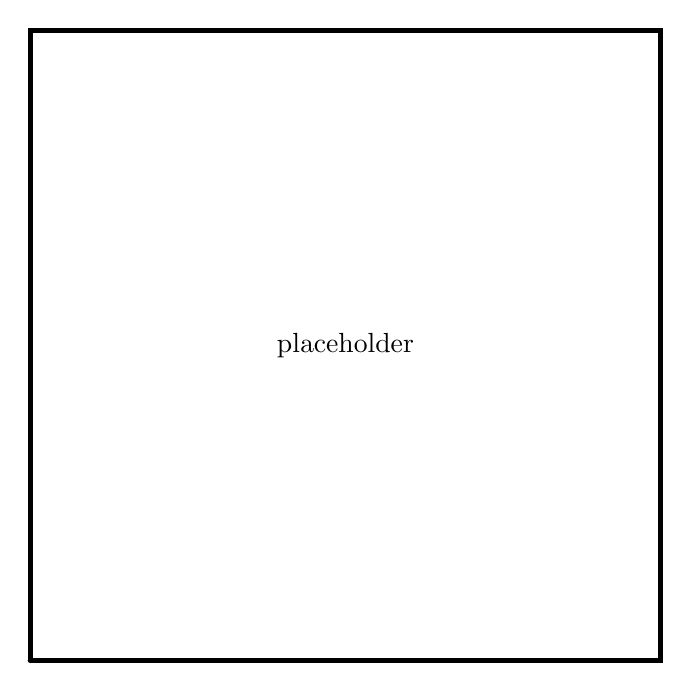
\begin{tikzpicture}[scale=2,cap=round,>=latex]
	\draw [line width=2] (-2, -2) -- (-2, 2) -- (2, 2) -- (2, -2) -- (-2, -2);
	
	\node at (0, 0) {placeholder};
\end{tikzpicture}
			\caption{Graphical solution to \ref{antisymtranceq}}
		\end{figure}
		
		In the limit case of $U_0 \rightarrow \infty$,
		\begin{align}
			\frac{k}{\kappa} =& -\tan(\frac{kd}{2}),\qquad \kappa \rightarrow \infty \Rightarrow \\
			\tan(\frac{kd}{2}) =& 0 \Rightarrow\qquad	\sin(\frac{kd}{2}) = 0 \Rightarrow\\
			\frac{kd}{2} =& \pi n \\
			k_n =& \frac{2\pi n}{d} \\
			E_n =& \frac{\hbar^2}{2m}\frac{1}{d^2}\left(2\pi n\right)^2
		\end{align}
		Which corresponds to antisymmetric solutions found earlier to the infinite quantum well problem.		
		
		\begin{figure}[!h]
			\centering
			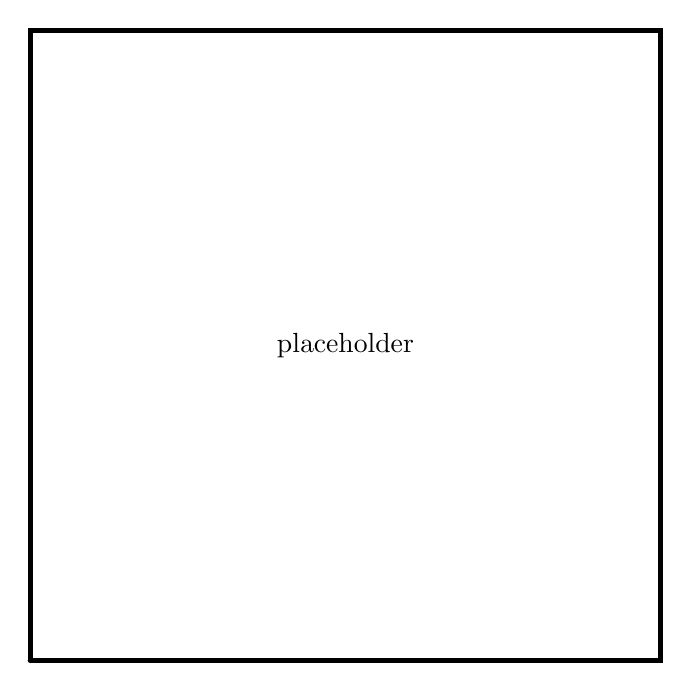
\begin{tikzpicture}[scale=2,cap=round,>=latex]
	\draw [line width=2] (-2, -2) -- (-2, 2) -- (2, 2) -- (2, -2) -- (-2, -2);
	
	\node at (0, 0) {placeholder};
\end{tikzpicture}
			\caption{Quantum well bound state wave functions}
		\end{figure}		
	\subsection{Harmonic oscillator}
	\subsection{Spherically symmetric potential}
	\subsection{Problems}
		\subsubsection{Rectangular quantum well}
			Double quantum well
			
			Double quantum barrier
			
			Minimal transistor size
			
			